
\section{Finger-Knuckle 2018 Project}

I have counted that the size of the split image is $208\times184$, then I resize all the segmented finger knuckle image to $208\times184$ while keep the image ratio. As for the feature of finger knuckle from neck part of YOLOv5. We can get outputs feature maps of three different sizes, 1/8 of the input image (Stride 8), 1/16 of the input image (Stride 16), and 1/32 of the input image (Stride 32) from the neck part. On these stride feature, we use the predicted finger knuckle bounding boxes to crop the finger knuckle feature maps, then using ROI Align to resize the same size. As for the Stride 8, I resize it to $26\times22$, and $14\times12$ and $8\times7$ for Stride 16 and Stride 32, respectively. I use the middle finger of left hand as the training set and test performance on the rest finger of left hand.


\subsection{Only use the segmented finger knuckle as the input of DoN 
model}
I use the DoN model to test its performance on my segmented finger knuckle, as shown on the Fig. \ref{don-roc}.

\begin{figure}[h]
    \centering
    \subfloat[]{
        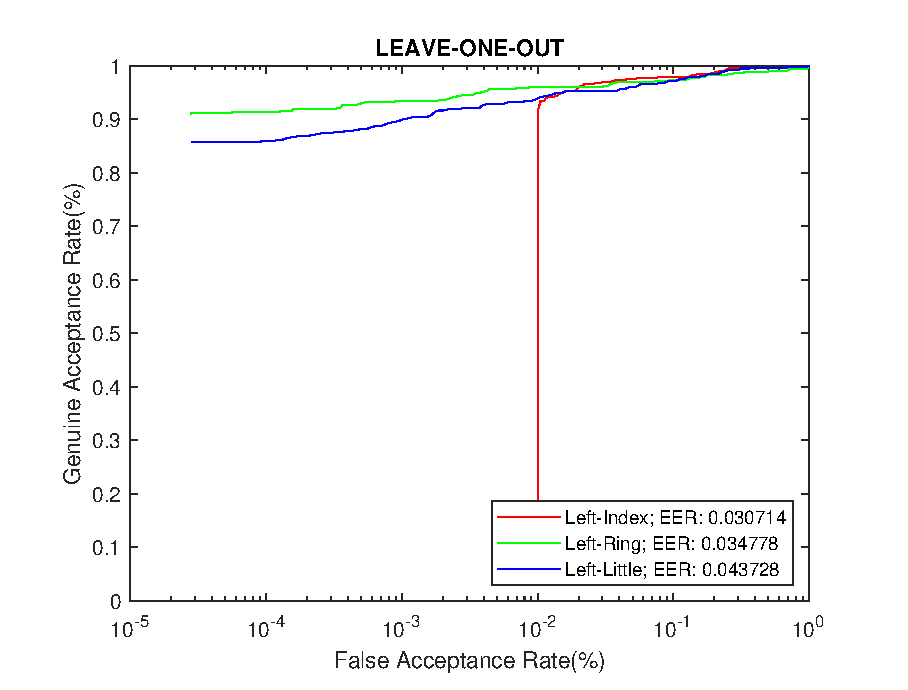
\includegraphics[width=2in]{Figure/04-11-2022/don-leave-one-out.eps}
        \label{}}
    \subfloat[]{
        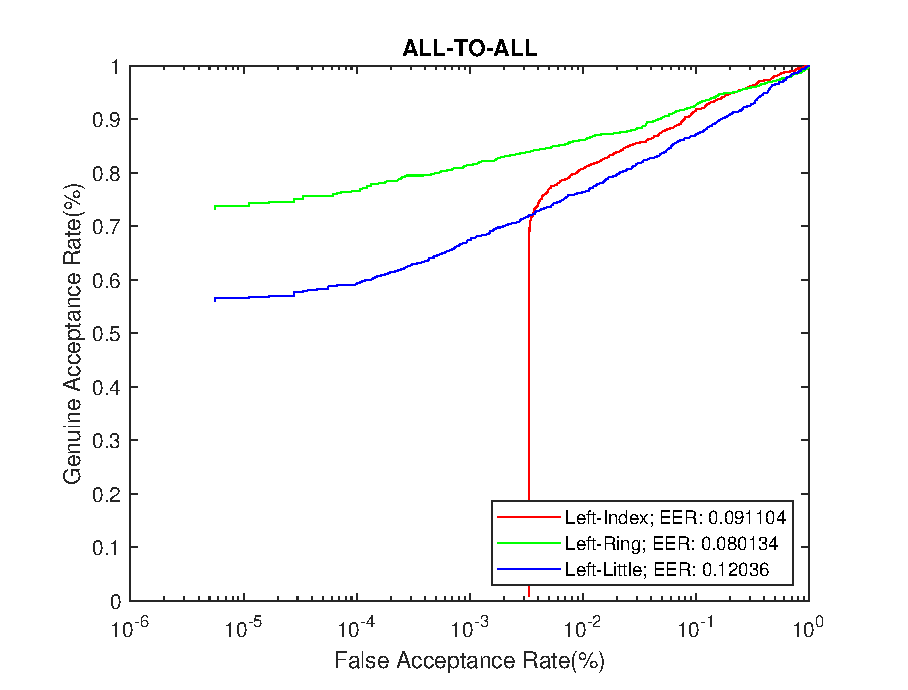
\includegraphics[width=2in]{Figure/04-11-2022/don-all-to-all.eps}
        \label{}}

    \caption{Matching performance with (a) leave-one-out protocol (b) all-to-all protocol}
    \label{don-roc}
\end{figure}




\subsection{Only use the segmented finger knuckle as the input of RFN model}

In the beginning, I plan to use the EfficientNet as the backbone for extracting feature maps. But the EfficientNet is too heavy result in costing a lot of GPU memory, and the performance is also lower than RFN.RFN performance can be shown as Fig. \ref{rfn-roc}.

\begin{figure}[h]
    \centering
    \subfloat[]{
        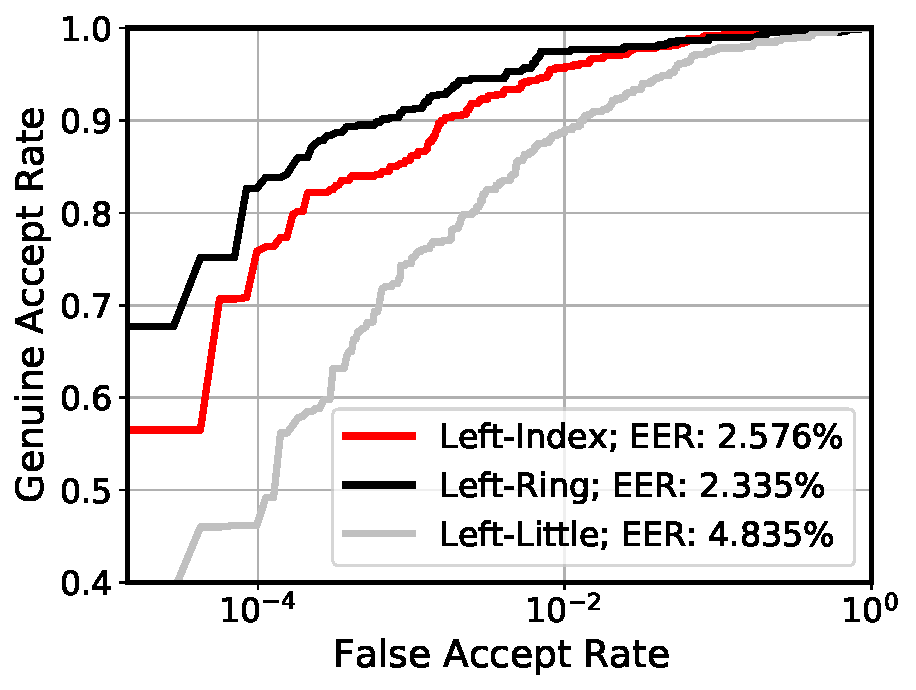
\includegraphics[width=2in]{Figure/04-11-2022/rfn-mse-leave-one-out-roc.pdf}
        \label{}}
    \subfloat[]{
        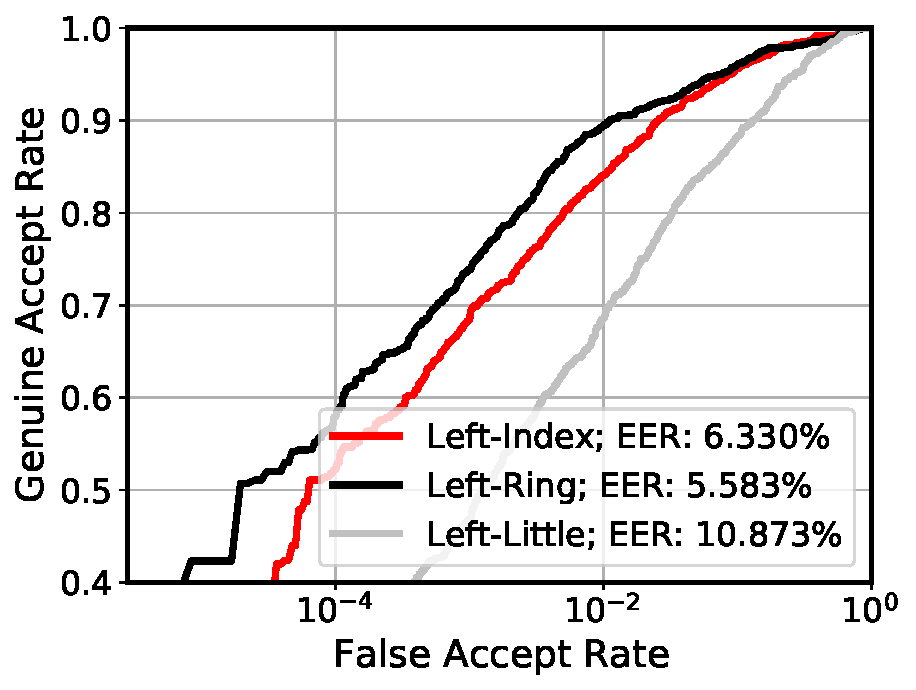
\includegraphics[width=2in]{Figure/04-11-2022/rfn-mse-all-to-all-roc.pdf}
        \label{}}

    \caption{Matching performance of RFN with (a) leave-one-out protocol, (b) all-to-all protocol}
    \label{rfn-roc}
\end{figure}

\subsection{Fuse feature maps from YOLOv5}

\begin{figure}[ht!]
    \centering
    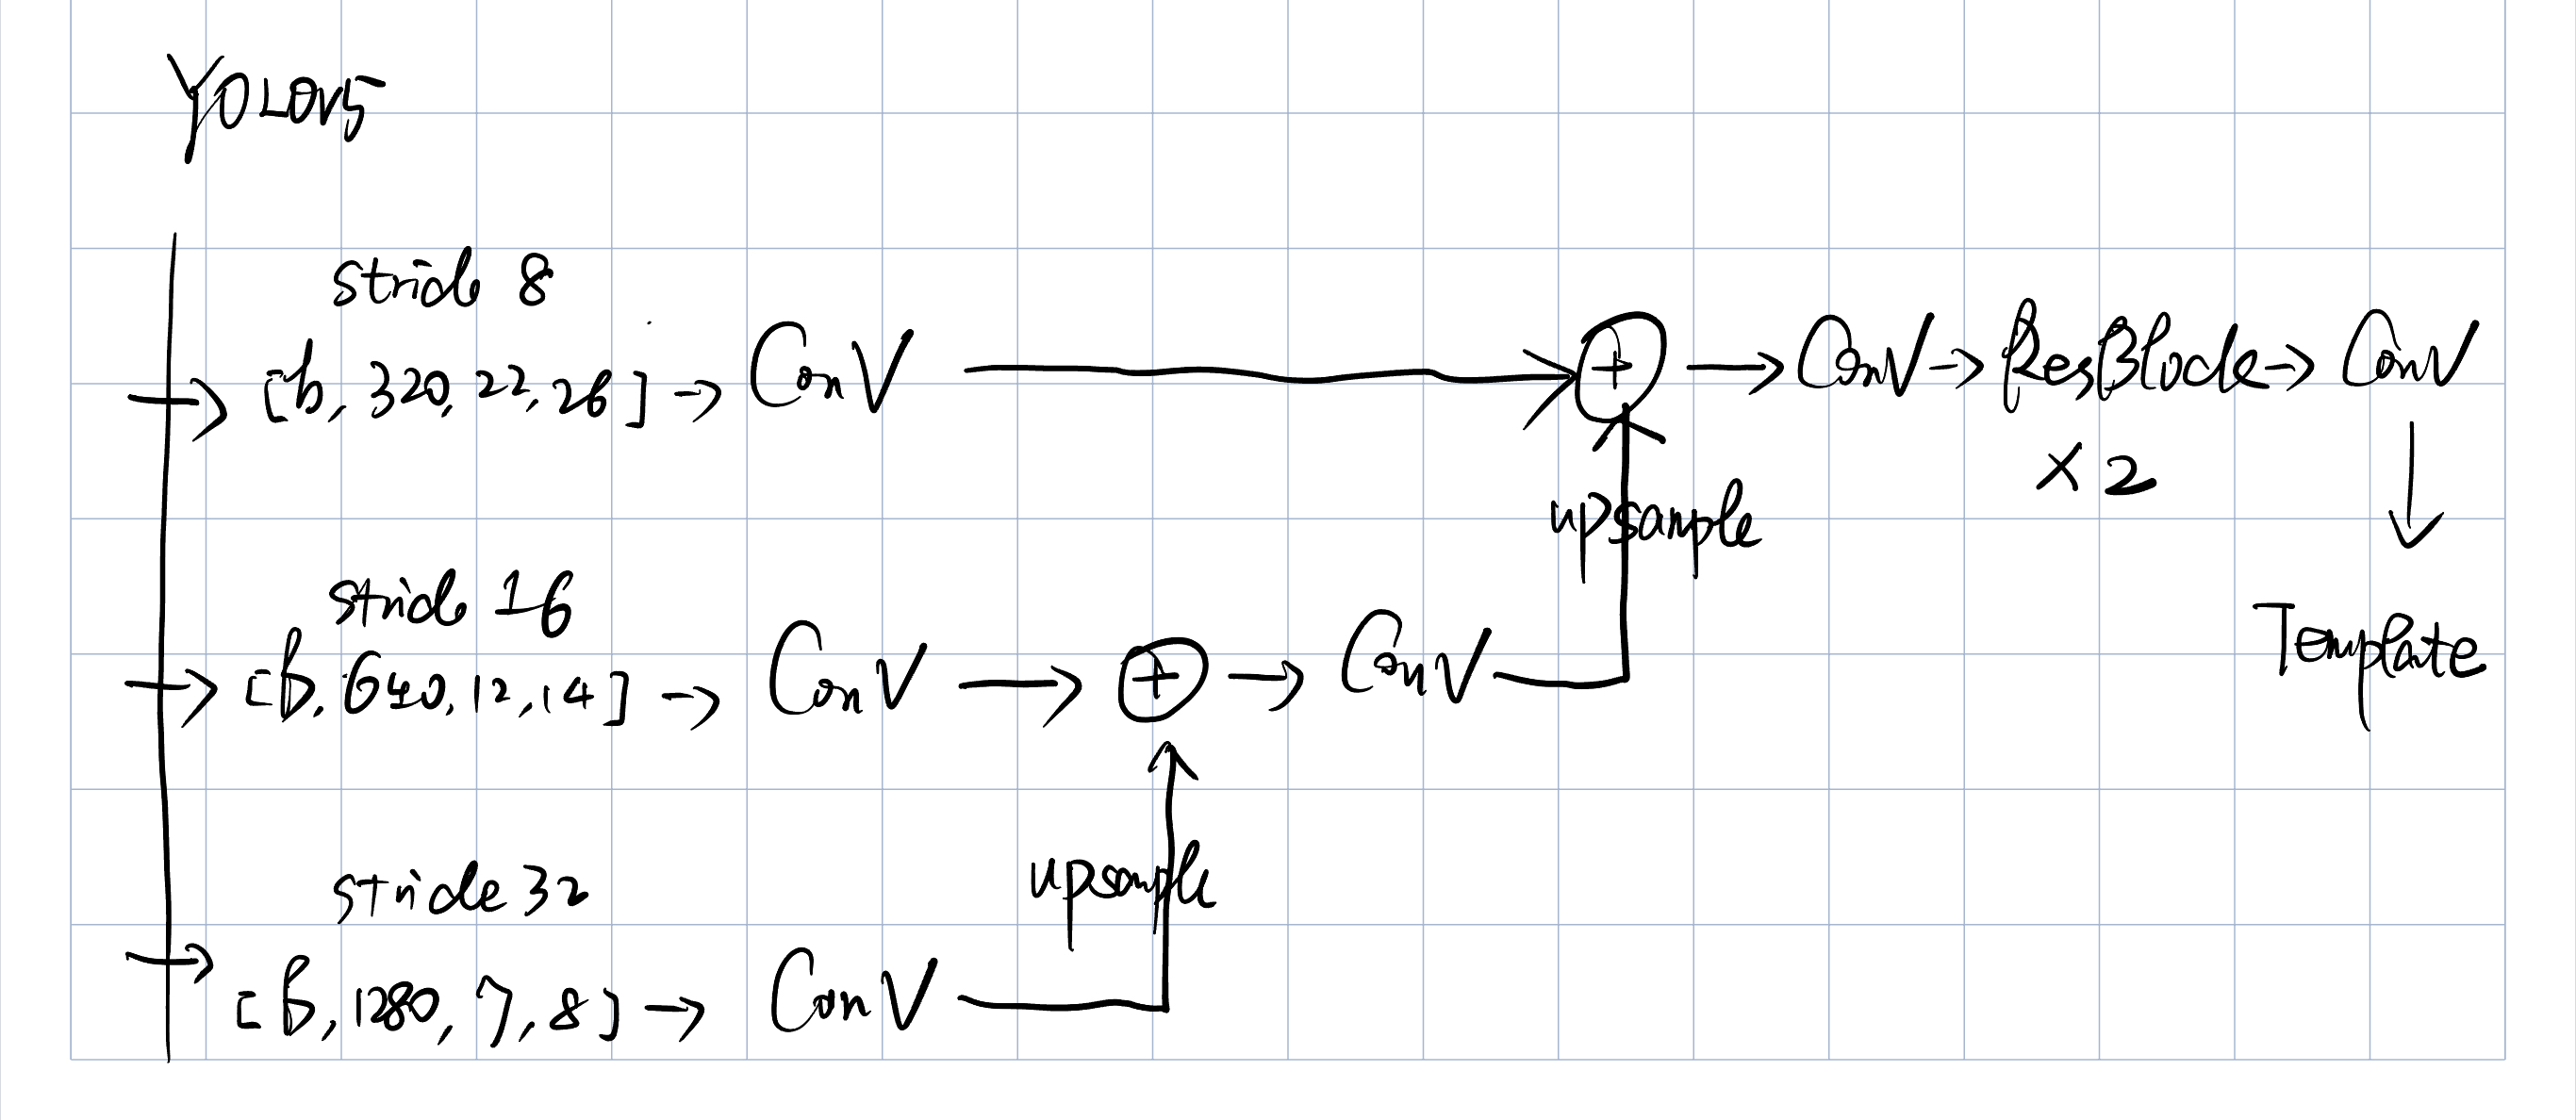
\includegraphics[width=3in]{Figure/04-11-2022/assistantmodel.jpg}
    \caption{The architecture of fusing 3 different output features from YOLOv5.}
    \label{assistantmodel}
\end{figure}

I have also tried its performance by fusing 3 different features and get the last features.
\begin{figure}[h]
    \centering
    \subfloat[]{
        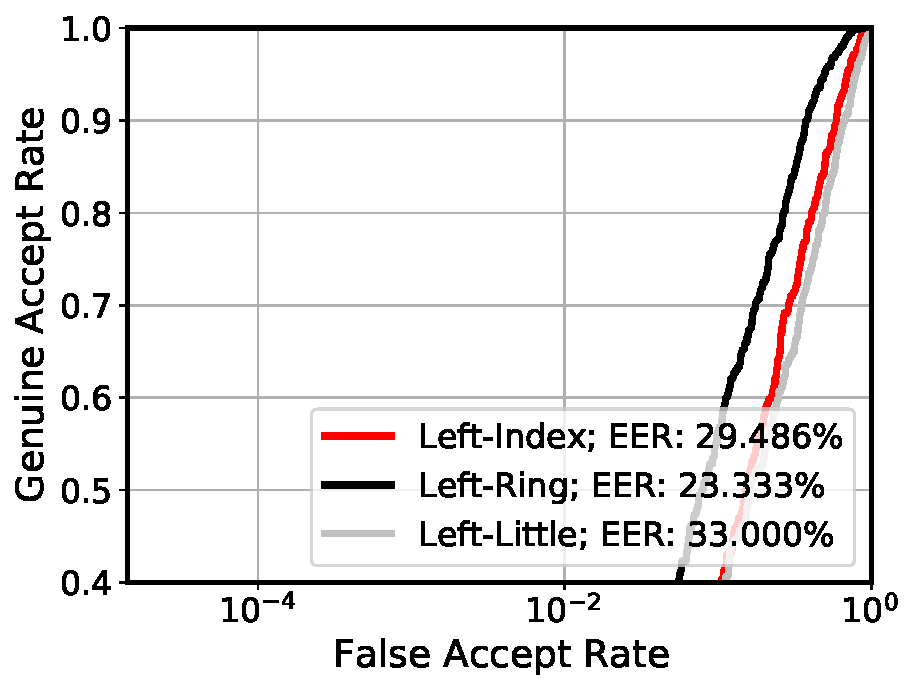
\includegraphics[width=2in]{Figure/04-11-2022/assistantmodel-leave-one-out-roc.pdf}
        \label{}}
    \subfloat[]{
        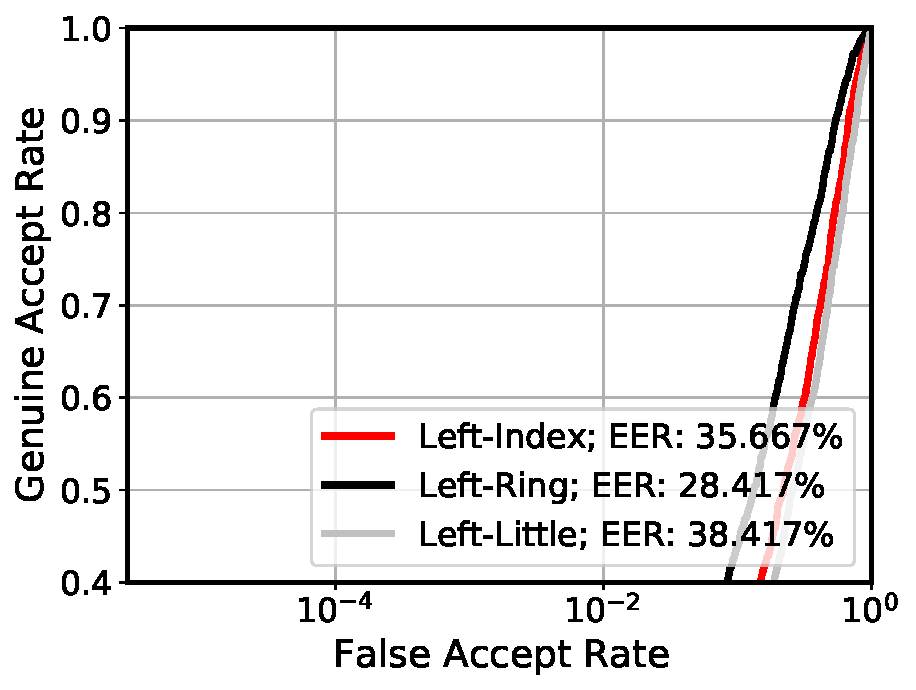
\includegraphics[width=2in]{Figure/04-11-2022/assistantmode-all-to-all-roc.pdf}
        \label{}}

    \caption{Matching performance of AssistantModel with (a) leave-one-out protocol, (b) all-to-all protocol}
    \label{fusionmodel-roc}
\end{figure}




\subsection{Fuse feature maps from YOLOv5 and segmented finger knuckle images}

\begin{figure}[ht!]
    \centering
    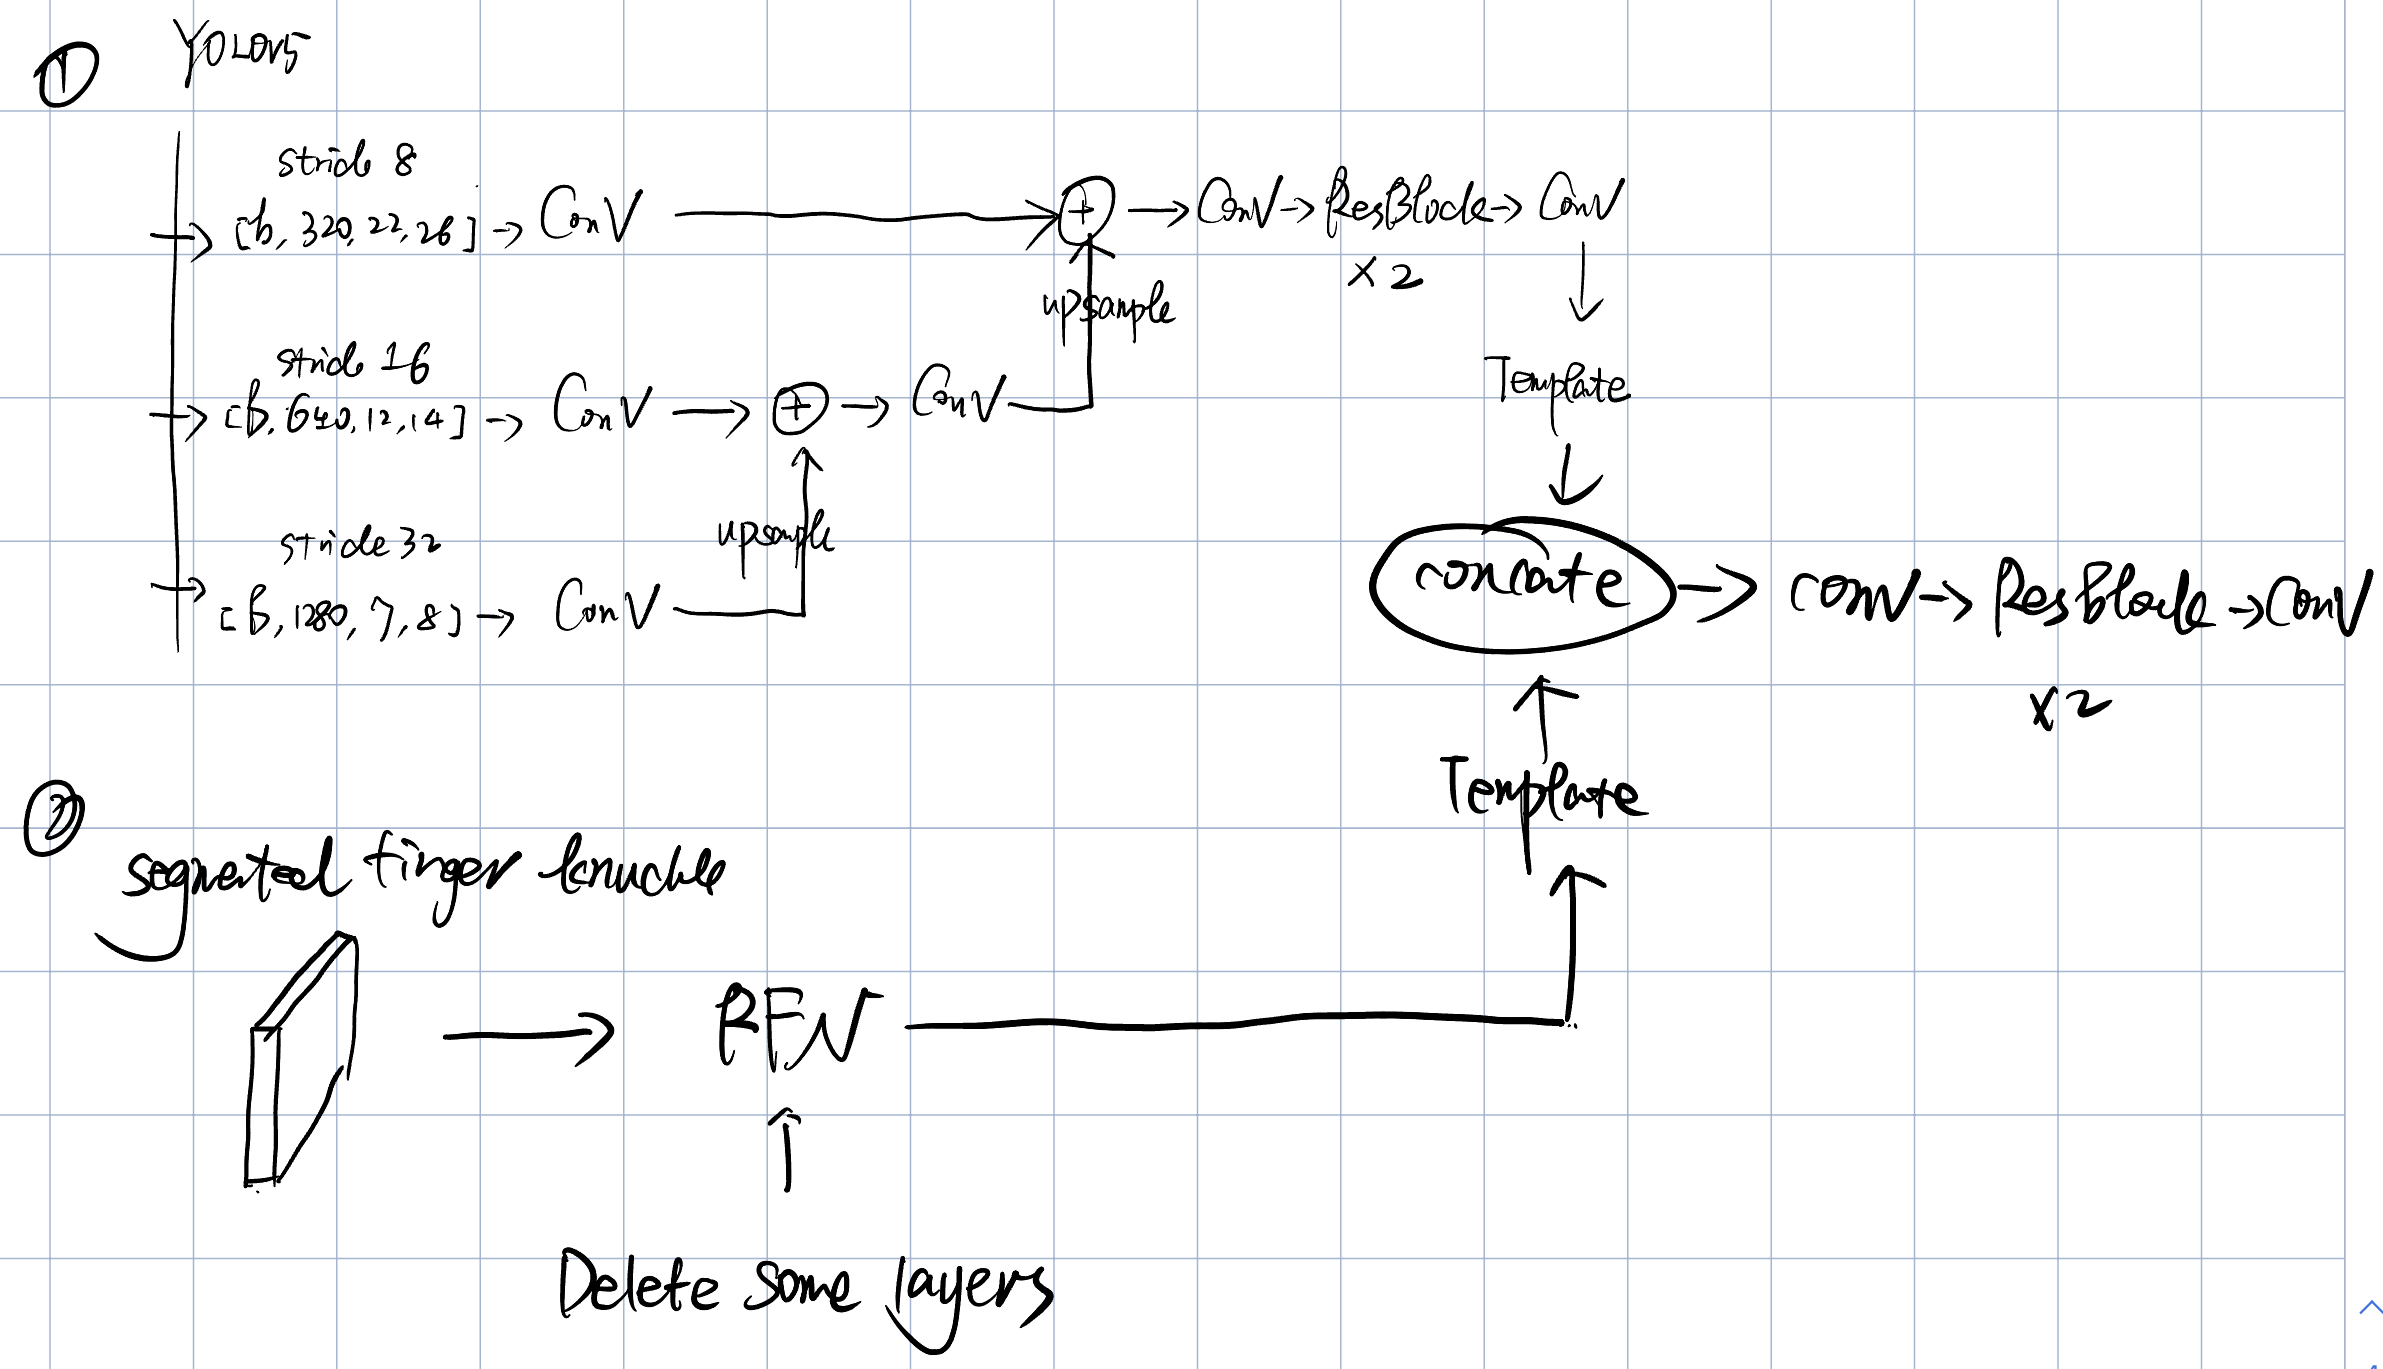
\includegraphics[width=4in]{Figure/04-11-2022/fusionmodel.jpg}
    \caption{The architecture of fusing features of YOLOv5 and segmented finger knuckle.}
    \label{fusionmodel}
\end{figure}

\begin{figure}[h]
    \centering
    \subfloat[]{
        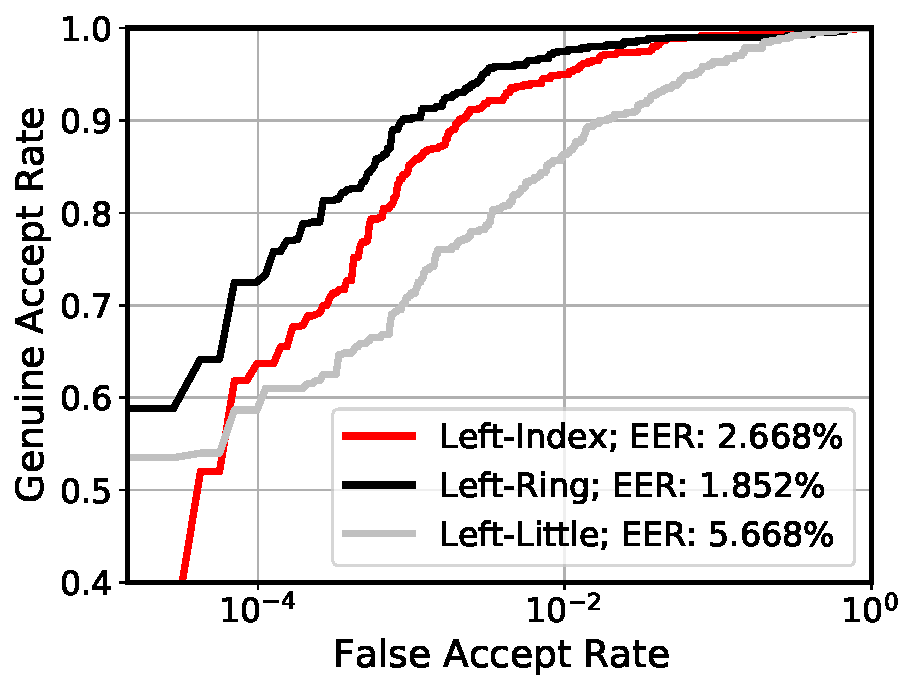
\includegraphics[width=2in]{Figure/04-11-2022/fusion-20-leave-one-out-roc.pdf}
        \label{}}
    \subfloat[]{
        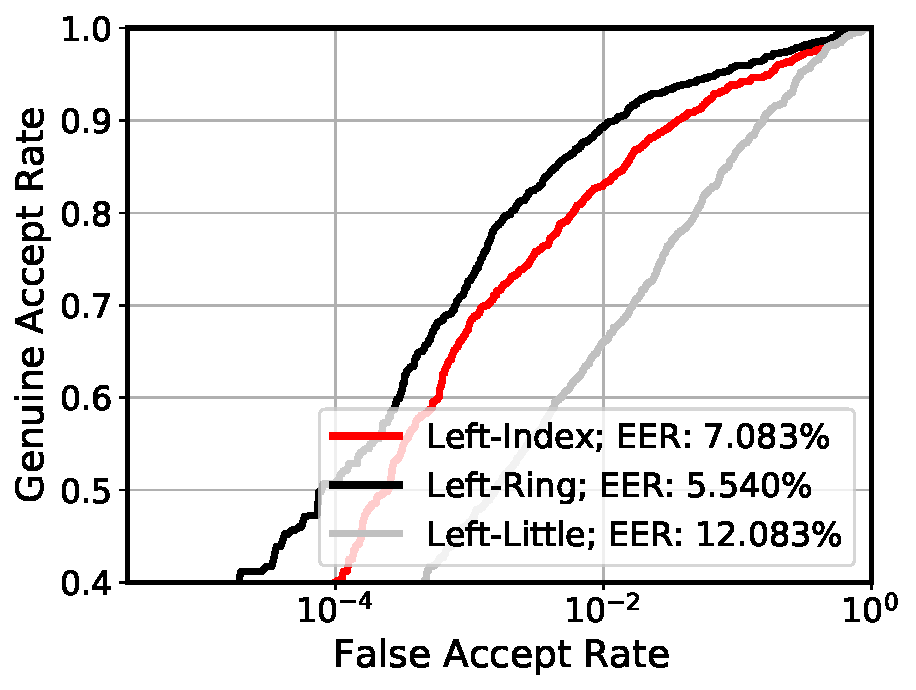
\includegraphics[width=2in]{Figure/04-11-2022/fusion-20-all-t0-all-roc.pdf}
        \label{}}

    \caption{Matching performance of FUsionModel with (a) leave-one-out protocol, (b) all-to-all protocol}
    \label{fusionmodel-roc}
\end{figure}